
\documentclass[a4paper]{article}
\usepackage[pdftex]{graphicx}
\usepackage[utf8]{inputenc}
\usepackage{enumerate}
\usepackage{siunitx}
\sisetup{locale=DE} 
\usepackage{icomma}
\usepackage{amssymb}
\usepackage{tikz}
\usepackage{href-ul}
\hypersetup{
	colorlinks=true,
	linkcolor=blue,
	urlcolor=blue}
\usepackage{geometry}
\geometry{a4paper, top=15mm, left=15mm, right=15mm, bottom=15mm,
	headsep=10mm, footskip=12mm}

\begin{document}
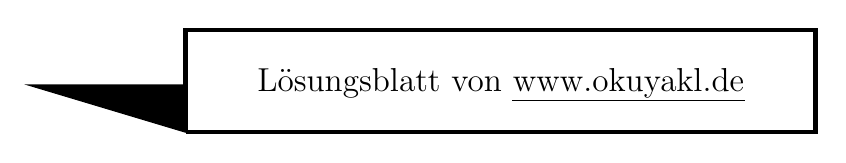
\begin{tikzpicture}(10,3)
	\draw[ultra thick](2,0) --(10,0) -- (10,1.3) --(2,1.3) -- (2,0);
	\draw[fill=black](2,0)-- (0,.6) -- (2,.6) -- (2,0);
	\node at (6,.6) {\large Lösungsblatt von \href{https://www.okuyakl.de}{www.okuyakl.de}};
\end{tikzpicture}
\vspace{0.5 cm}

\begin{minipage}{0.5\textwidth}
{\bf Aufgabe 1. a)}\\
\includegraphics[width=6 cm]{ikurv235.png}	
\end{minipage}
\hfill
\begin{minipage}{0.5\textwidth}
{\bf Aufgabe 1. b)}\\
Die Stromstärke ist maximal zu dem Zeitpunkt, an welchem der Kondensator entladen ist. Mit weiterem, nun abnehmenden Stromfluss lädt sich der Kondensator bis zu dem Zeitpunkt, an dem der Stromfluss seine Nullstelle erreicht.
\end{minipage}
\vspace{0.5 cm}

\noindent{\bf Aufgabe 1. c)}\\
Wir betrachten die Gesamtenergie, während sie als magnetische Energie in der Spule vereinigt ist, und setzen:
$$
\renewcommand{\arraystretch}{2}
\begin{array}{rcll}
 W_{ges}&=&{1 \over 2} L \cdot I^2 &|\cdot 2 : I^2\\
 {2 \cdot W_{ges}\over I^2} &=& L \\
 L &=&  {2 \cdot \SI{2,9e-3}{\watt}  \over (\SI{0,12}{\ampere})^2} &= \SI{0,40}{\henry}
\end{array}
$$  
Mit der Thomsongleichung erhalten wir nun $C$:
$$
\renewcommand{\arraystretch}{2}
\begin{array}{rcll}
  T &=& 2 \pi \sqrt{LC} &| ()^2\\
T^2 &=& 4 \pi^2 LC & |: 4 \pi^2 L \\
  C &=& { T^2 \over 4 \pi^2 L} \\
  C &=& { (\SI{2,0e-3}{\second})^2 \over 4 \pi \cdot \SI{0,40}{\henry}} \\
  C &=& \SI{2,5e-7}{\farad}&=\SI{0,25}{\micro\farad}  
\end{array}
$$  
\vspace{0.5 cm}

\noindent{\bf Aufgabe 1. d)}\\
Die maximale Ladung entspricht der Fläche unter der Kurve während der Ladezeit des Kondensators. Somit ist $Q_{max}$:
$$
\renewcommand{\arraystretch}{2}
\begin{array}{rcll}
Q_{max} &=& \int\limits_{t_1}^{t_2}I(t)dt\\
Q_{max} &=& \int\limits_{\SI{0,5}{\milli\second}}^{\SI{1,0}{\milli\second}}\SI{0,12}{\ampere} \cdot \sin{\left({2\pi \over \SI{2,0}{\milli\second}}\right) \cdot t}dt \\
Q_{max} &=& \left[\SI{-0,12}{\ampere} \cdot{\SI{2,0}{\milli\second}\over 2\pi} \cos{\left(2\pi \over \SI{2,0}{\milli\second}\right)\cdot t} \right]_{\SI{0,5}{\milli\second}}^{\SI{1,0}{\milli\second}}\\
Q_{max} &=& \SI{3,8e-5}{\coulomb}
\end{array}
$$  
\vspace{0.5 cm}

\noindent{\bf Aufgabe 1. e)}\\
Die Gesamtenergie setzt sich zusammen aus Energie des Kondensators und Energie der Spule:
$$ 
\renewcommand{\arraystretch}{2}
\begin{array}{rcll}
W_{ges} & = & W_{K} + W_{Sp} &| - W_{Sp}\\
W_{K}   & = & W_{ges}-  {1 \over 2} LI^2\\
W_{K}   & = & \SI{2,9e-3}{\joule}  - {1 \over 2}\cdot \SI{0,40}{\henry} \cdot (\SI{0,090}{\ampere})^2\\
W_{K}   & = & \SI{0,0013}{\joule}
\end{array}
$$  
\vspace{0.5 cm}

\noindent{\bf Aufgabe 2. a)}\\
Die Länge des Dipols entspricht der halben Wellenlänge:
$$l_0 = {\lambda \over 2} = {c \over 2 f} = {\SI{3e8}{\meter\over \second}\over 2\cdot \SI{2,5e9}{\hertz}} = \SI{0,06}{\meter} $$
\vspace{0.5 cm}

\noindent{\bf Aufgabe 2. b)}\\
Das Hertzsche Gitter ist nur für Wellen durchlässig, die einen zu ihm senkrechten Anteil der Schwingungsebene besitzen. Im angeführten Fall ist das Gitter parallel zur Schwingungsebene, daher reflektiert es die Welle wie eine leitende Fläche. Der Empfangsdipol hinter dem Gitter empfängt kein Signal.
\vspace{0.5 cm}

\begin{minipage}{0.4\textwidth}
\noindent{\bf Aufgabe 2. c)}\\
	\includegraphics[width=5 cm]{hedi235.pdf}	
\end{minipage}
\hfill
\begin{minipage}{0.5\textwidth}
Der Empfangsdipol empfängt bei $0^\circ$ Gitterdrehung 0\%; bei $90^\circ$ Drehung 100\% des Signals. Dies legt nahe, eine Winkelfunktion zugrunde zu legen. Die wirksame Länge sei $l$
$$l = l_0 \cdot (1-\cos\alpha)$$
Die empfangene Leistung $P$ ist proportional zum Quadrat der wirksamen Länge $l$
$${P \over P_0} = 100\% \cdot (1-\cos 55^\circ)^2 =18\%$$
$D_E$ empfängt also nun 18\% des Signals.
\end{minipage}
\vspace{0.5 cm}

\begin{center}
	\includegraphics[width=7 cm]{../../viecher/endcomic.pdf}
	
	Hier geht es zurück zum \href{https://www.okuyakl.de/phys/p13schikL235/aa235.pdf}{Aufgabenblatt}
\end{center}

\end{document}